\section{Funktionsweise von Simulink}
Simulink ist eine auf Blockschaltbildern basierende Programmierplattform, welche ursprünglich dazu gedacht war Differentialgleichungen numerisch zu lösen und Simulationen durchzuführen. Im Verlauf der Zeit wurde diese Basis kontinuierlich erweitert und unterstützt mittlerweile zahlreiche Funktionen. Eine bemerkenswerte Funktionalität von Simulink ist die Generation von Quellcode für Microcontroller. Damit können sowohl in kurzer Zeit umfangreiche Applikationen entworfen werden als auch durch Kommunikationsprotokolle zwischen Host- und Target-Plattform HiL-, SiL- und PiL-Simulationen durchgeführt werden. Somit stellt es ein mächtiges Werkzeug dar um Hardwarebausteine wie Sensoren und Microcontroller auszuwerten und daraufhin Filter und Regelungssysteme zu entwerfen.

In den folgenden Abschnitten werden die verschiedenen Ausführungsmodi und der Simulationsprozess von Simulink näher erklärt.

\subsection{Ablauf einer Simulink-Simulation}
Der Ablauf einer Simulation läuft in verschiedenen Phasen ab. Zuerst wird ein Model initialisiert. Hierbei werden die Datentypen, Weiten und Abtastraten der Blöcke und Signale festgelegt. Anschließend werden die Blockparameter ausgewertet und die Blockreihenfolge zur Ausführung bestimmt. Im nächsten Schritt wird die Simulation in einer Schleife ausgeführt. Das einmalige durchlaufen dieser Schleife wird auch als Simulationsschritt (Simulation step) bezeichnet. Der Aufbau der Simulationsschleife hängt von den Eigenschaften des Modelles ab. Besitzt ein Simulink-Modelle Blöcke mit variablen Abtastraten wird vor jedem Simulationsschritt dessen Ausführungszeitpunkt berechnet. Bei einem Modell fixen Abtastraten wird diese Berechnung nicht benötigt. Außerdem wird zwischen Blöcken mit diskreten und kontinuierlichen Zuständen unterschieden. Ein Block mit diskreten Zuständen wird einmal pro Simulationsschritt aufgerufen um seinen, für diesen Simulationsschritt, aktuellen Zustand und Ausgangswerte zu berechnen. Bei einem Block mit kontinuierlichen Zuständen wird dieser mit einer höheren Abtastrate als das restliche Model aufgerufen. In diesen Aufrufen werden die aktuellen Ausgangswerte und Ableitungen des Blocks berechnet.

\begin{figure}[h]
	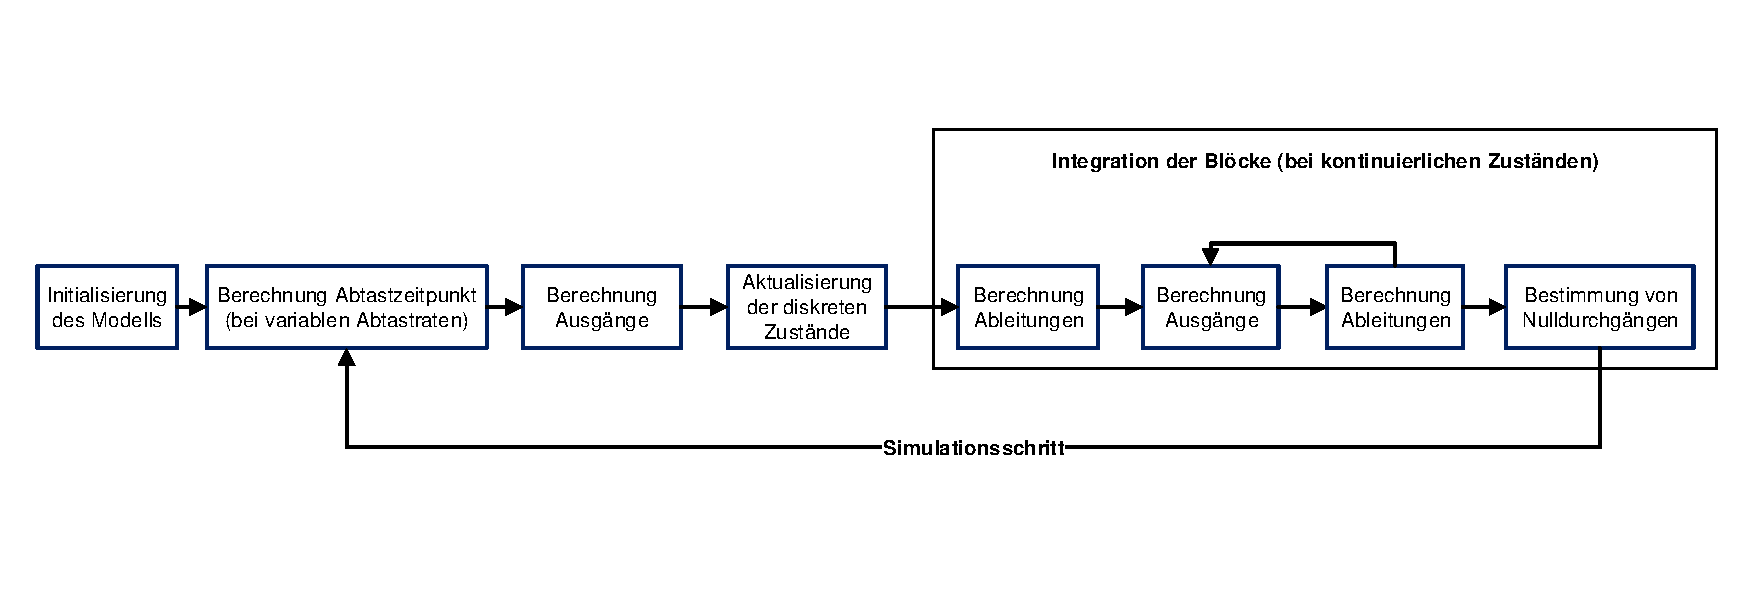
\includegraphics[width=\linewidth]{AblaufSimulation}
	\caption{Ablauf einer Simulation, Quelle: eigene Darstellung, Inhalt aus \cite{SFunc}}
\end{figure}

\subsection{Aufbau eines Simulink-Blocks}
Ein Simulink-Block muss Funktionen bereitstellen um die oben genannten Schritte einer Simulation zu ermöglichen. Darunter fallen die Folgenden Funktionen:

\begin{itemize}
	\item Initialisierung des Blocks
	\item Berechnung des nächsten Abtastzeitpunktes (falls der Block variable Abtastraten benötigt)
	\item Berechnung der Ausgangswerte
	\item Berechnung der diskreten Zustände des Blocks
	\item Integration, hierunter fallen die Berechnung der Ausgangswerte und Ableitungen bei Zwischenschritten (wird nur bei kontinuierlichen Zuständen benötigt)
\end{itemize}

Die Umsetzung dieser Methoden erfolgt in der Form einer sogenannten \textit{S-Function}. Hierbei handelt es sich lediglich um eine Sammlung von Funktionen, welche die oben genannten Aktionen implementieren. Eine \textit{S-Function} kann in unterschiedlichen Programmiersprachen implementiert werden, wobei MATLAB und C/C++ die üblichsten sind. Hier sollen lediglich \textit{S-Functions} in C/C++ vorgestellt werden, in \cite{SFunc} werden alle Alternativ detailliert erklärt. 